\documentclass[10pt,twocolumn]{article}
\usepackage[margin=0.72in]{geometry}
\usepackage{amsmath,amssymb,booktabs,graphicx,hyperref}
\title{\textbf{Hardened Compiler Passes, Exact 256-Branch \& 16/16 Fault-Taxonomy Verification, RFC 8785 Execution Ledger, and Hash-Locked Quantinuum H2 Dispatch for 20-Qubit Toroidal Wen-Plaquette Feed-Forward Preparation}}
\author{Devin Phillip Davis\\Agile Defense Systems LLC\\\texttt{v1.1.0 DOI: 10.5281/zenodo.24421051} \quad \texttt{v1.0.0 DOI: 10.5281/zenodo.24406733} \quad \texttt{https://github.com/quantum-osiris/osiris-qec}}
\date{November 21, 2026 --- Version 1.1.0 (\textbf{STATUS: HARDWARE-UNVALIDATED})}

\begin{document}
\maketitle

\begin{abstract}
\noindent\textbf{Status: HARDWARE-UNVALIDATED.} Compilation and execution use a preregistered artifact lock: the pre-compile SHA-256 (\texttt{b86aeabd70eecb7f5fbc...}) and Quantinuum H2-1 ISA SHA-256 (\texttt{02d5cb72849f9b473c02...}) are verified immediately prior to execution and post-compile under \texttt{optimisation\_level=0}; any mismatch invalidates the run and aborts submission. Building upon the prior-art $4\times 4$ toroidal Wen-plaquette two-round LUT protocol of Iqbal \emph{et al.} (arXiv:2302.01917), OSIRIS-QEC v1.1.0 preserves the immutable v1.0.0 baseline (\texttt{10.5281/zenodo.24406733}) while adding strict register-collision protection, metadata normalization, a complete $16/16$ post-preparation Pauli-$Y$ sweep, an IETF RFC~8785 hash-chained write-ahead execution ledger, and the \texttt{osiris qec} CLI for Selene validation and hash-locked Quantinuum H2-1 dispatch.
\end{abstract}

\section{Hardware Allocation and Pass Hardening}
Sixteen data qubits $q[0..15]$ implement the $[[16,2,4]]$ toroidal Wen-plaquette encoding, while $4$ ancilla qubits $q[16..19]$ are recycled via mid-circuit \texttt{Reset} ($24$ \texttt{Measure}, $8$ \texttt{Reset} total; ancillas do not contribute to logical code distance; Fig.~\ref{fig:torus}). \texttt{WenPlaquetteFeedForwardPass} and \texttt{build\_wen\_plaquette} reject non-empty inputs and colliding \texttt{q/qr/quantum/c/creg/cl/classical} registers while normalizing mutable metadata so v1.0.0 and v1.1.0 circuit hashes match bit-for-bit.

\begin{figure}[t]
\centering
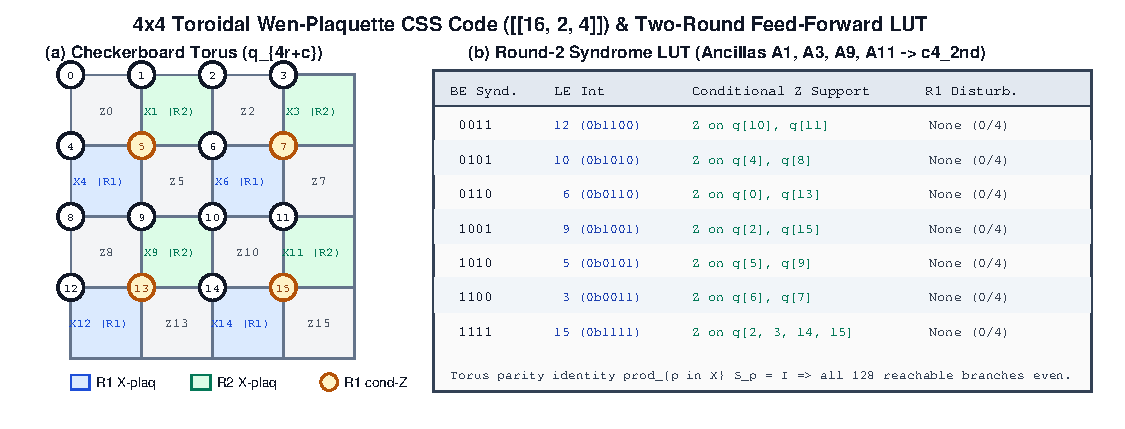
\includegraphics[width=\columnwidth]{fig1_torus_checkerboard_lut.pdf}
\caption{$[[16,2,4]]$ toroidal layout ($16$ data + $4$ recycled ancillas) and $7$-entry Round-2 LUT.}
\label{fig:torus}
\end{figure}

\section{Exact Verification and Noise Benchmark}
Exhaustive $256$-branch enumeration confirms $128/128$ reachable even-parity branches land in $+1$ codespace (worst $\langle S\rangle = 0.9999999999999942$), cross-checked in $X$ ($512/512$) and $Z$ ($256/256$) bases on Qiskit Aer and via \texttt{osiris qec run --target selene}. Table~\ref{tab:bench} and Fig.~\ref{fig:bench} report noisy trajectories.

\begin{figure}[t]
\centering
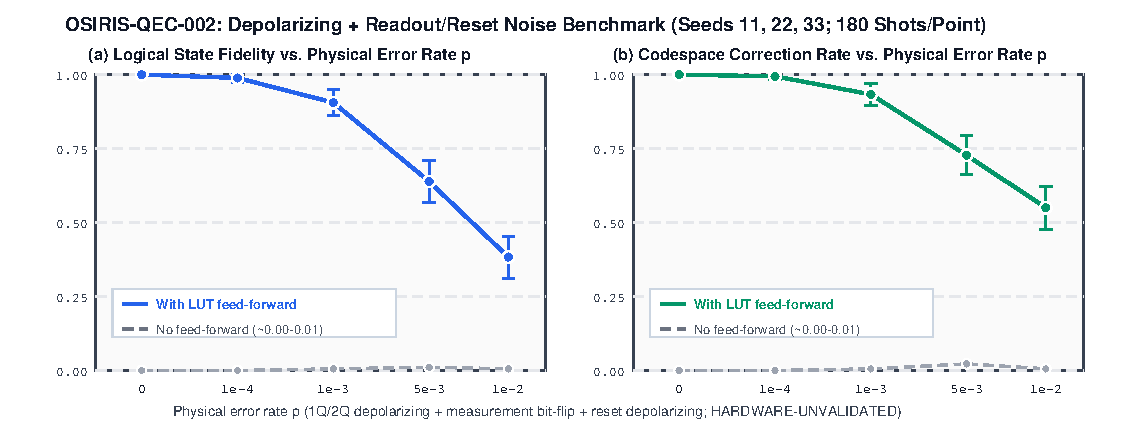
\includegraphics[width=\columnwidth]{fig2_noisy_fidelity_benchmark.pdf}
\caption{Simulated depolarizing + readout/reset noise benchmark ($180$ shots/point).}
\label{fig:bench}
\end{figure}

\begin{table}[t]
\centering
\caption{Pooled noisy preparation benchmark (simulation only).}
\label{tab:bench}
\footnotesize
\begin{tabular}{ccccc}
\toprule
$p$ & Shots & FF Fidelity & FF Codespace & No-FF Fid. \\
\midrule
0 & 180 & $1.0000 \pm 0.0000$ & $1.0000 \pm 0.0000$ & $0.0000$ \\
0.0001 & 180 & $0.9889 \pm 0.0153$ & $0.9944 \pm 0.0109$ & $0.0000$ \\
0.001 & 180 & $0.9056 \pm 0.0427$ & $0.9333 \pm 0.0364$ & $0.0056$ \\
0.005 & 180 & $0.6389 \pm 0.0702$ & $0.7278 \pm 0.0650$ & $0.0111$ \\
0.01 & 180 & $0.3833 \pm 0.0710$ & $0.5500 \pm 0.0727$ & $0.0056$ \\
\bottomrule
\end{tabular}
\end{table}

\section{16/16 Post-Prep Fault Taxonomy \& Hash-Locked H2 Gate}
Expanding post-preparation $Y$-fault injection to all $16/16$ data qubits confirms $16/16$ partial $X$-syndrome detection with $0/16$ preservation ($F_L=0.0$; Fig.~\ref{fig:gate}). \texttt{osiris qec} enforces RFC~8785 write-ahead ledgering, \texttt{optimisation\_level=0}, post-compile ISA hash verification, and the $95\%$ Wilson lower bound $>0.99$.

\begin{figure}[t]
\centering
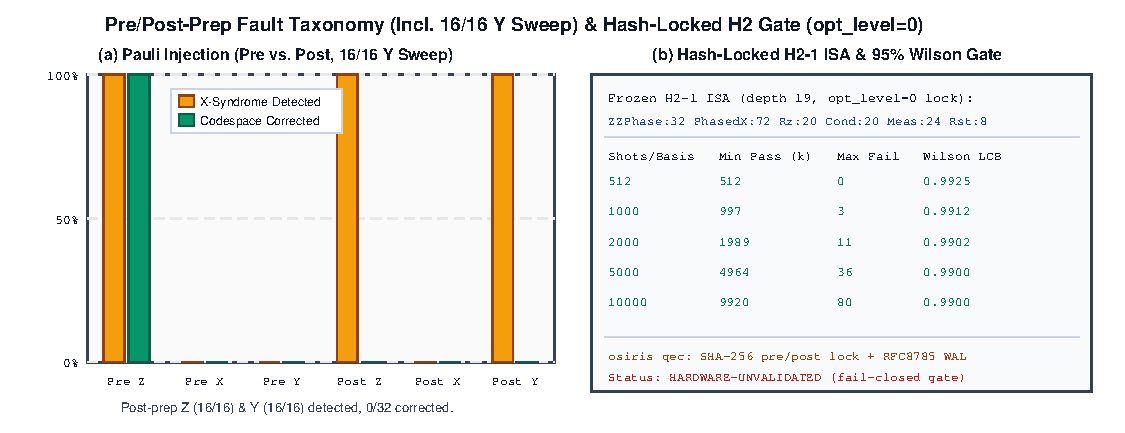
\includegraphics[width=\columnwidth]{fig3_error_taxonomy_and_wilson_gate.pdf}
\caption{$16/16$ pre/post-prep Pauli taxonomy and hash-locked Quantinuum H2 Wilson ($>0.99$) gate.}
\label{fig:gate}
\end{figure}

\begin{thebibliography}{9}
\bibitem{Iqbal2024} M. Iqbal \emph{et al.}, Commun.\ Phys.\ \textbf{7}, 205 (2024); arXiv:2302.01917.
\bibitem{Wen2003} X.-G. Wen, Phys.\ Rev.\ Lett.\ \textbf{90}, 016803 (2003).
\bibitem{RFC8785} A. Rundgren \emph{et al.}, IETF RFC 8785 (2020).
\bibitem{Wilson1927} E. B. Wilson, J.\ Am.\ Stat.\ Assoc.\ \textbf{22}, 209--212 (1927).
\bibitem{DavisV100} D. P. Davis, OSIRIS-QEC v1.0.0, Zenodo \texttt{10.5281/zenodo.24406733} (2026).
\end{thebibliography}
\end{document}
